\chapter{Programmazione Dinamica}

La tecnica della programmazione dinamica, come per la tecnica \textit{divide-et-impera}, è una tecnica di risoluzione di problemi andando ad dividere il problema in più sotto-problemi, questo però con la differenza che nella programmazione dinamica esiste la possibilità che uno o più sotto-problemi siano uguali tra loro, in questo caso si può sfruttare la tecnica della \textit{memorizzazione} per evitare di ricalcolare più volte lo stesso sotto-problema. Idealmente la soluzione a questo problema è quella di memorizzare i risultati dei sotto-problemi in una tabella, in modo da poterli riutilizzare successivamente, e il \textit{lookup} nella tabella deve essere in tempo $O(1)$.

\paragraph{Approccio Generale}
    \begin{figure}[H]
        \centering
        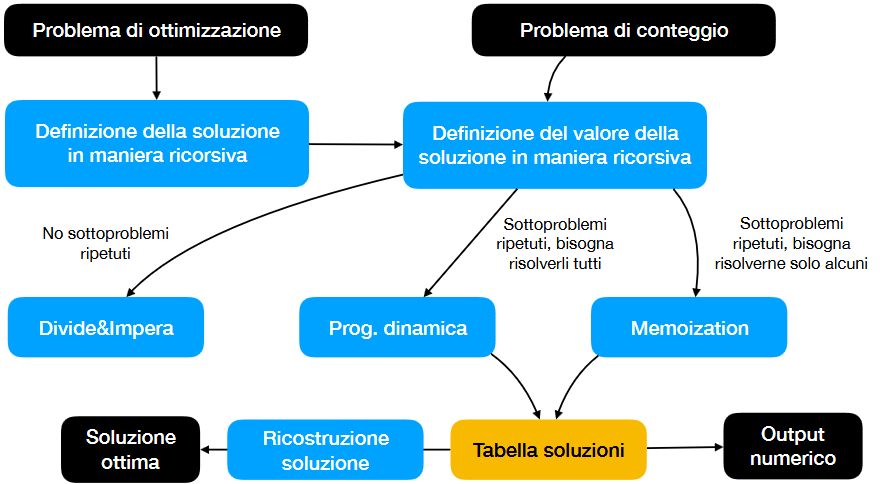
\includegraphics[width=0.6\textwidth]{10/approccioGenerale.png}
        \caption{Grafico dei passi da eseguire sulla base del tipo di problema}
    \end{figure}
    Se il problema è del tipo di ``ottimizzazione'' allora rispetto ai problemi del tipo ``conteggio'' deve essere definita una soluzione in maniera ricorsiva ``di base'' e una funzione di transizione che permetta di passare da un sotto-problema ad un altro. Fatto questo và definito il valore della soluzione in maniera ricorsiva se affrontando il calcolo non vengono rinvenuti sotto-problemi uguali, allora si usa la tecnica \textit{divide-et-impera}, altrimenti usiamo o la programmazione dinamica nel caso nel quale tutti i sotto-problemi vadano risolti, oppure la tecnica della \textit{memorization} nel caso nel quale non tutti i sotto-problemi vadano risolti.\newline
    Negli ultimi due casi non viene fornita immediatamente la soluzione, infatti viene prodotta una ``tabella delle soluzioni'' che nel caso dei problemi di conteggio conterrà il numero di soluzioni, mentre nel caso dei problemi di ottimizzazione bisognerà ricostruire la soluzione a partire dalla tabella delle soluzioni per ottenere la soluzione ottima.

\newpage
\section{Primi Problemi}
    Dopo aver visto l'approccio generale alla programmazione dinamica, vediamo ora alcuni problemi che possono essere risolti con questa tecnica.
    \subsection{Domino}
        Il problema del domino è un problema di conteggio, in cui si vuole contare il numero di modi in cui si possono posizionare $n$ tessere di domino in una scacchiera $2 \times n$ in modo che tutte le celle siano coperte da una tessera di domino. Ad esempio nel caso di $n=4$ allora il numero di modi in cui si possono posizionare le tessere è $5$.
        \begin{figure}[H]
            \centering
            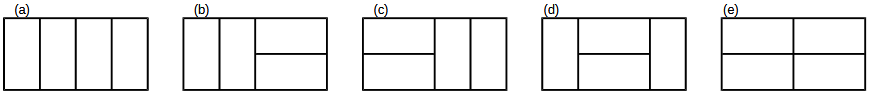
\includegraphics[width=0.8\textwidth]{10/domino.png}
            \caption{Esempio di posizionamento delle tessere di domino per il caso $n=4$}
        \end{figure}
        \subsubsection{Definizione ricorrenza}
            Definiamo una formula ricorsiva $DP[n]$ che definisce il numero di disposizioni possibili con $n$ tessere.
            \paragraph{Casi Base} Per fare ciò dobbiamo stabilire dei ``casi base''. Infatti per $n=0,1$ allora esiste solo $1$ disposizione possibile.
            \paragraph{Casi ricorsivi} Possiamo notare come nel caso nel quale posizionassimo l'ultima tessera in verticale allora le altre precedenti saranno disposte come per il caso $n-1$, mentre se la posiziono in orizzontale allora le precedenti saranno disposte come per il caso $n-2$ in quanto la penultima tessera deve essere posizionata in verticale. Dunque il caso $n$ sarà composto dal caso $n-1$ e dal caso $n-2$.
            \paragraph{Formula Ricorsiva} La formula ricorsiva sarà dunque:
            \begin{equation*}
                DP[n] = \begin{cases}
                    1 & n \leq 1 \\
                    DP[n-1] + DP[n-2] & n > 1
                \end{cases}
            \end{equation*}
            inoltre l'algoritmo ``naive'' per risolvere il problema ha la seguente struttura:
            \begin{algorithm}[H]
                \caption{\Int \texttt{domino1}(\Int $n$)}
                \begin{algorithmic}
                    \If{$n \leq 1$}
                        \State \Return $1$
                    \EndIf
                    \State \Return \texttt{domino1}($n-1$) + \texttt{domino1}($n-2$)
                \end{algorithmic}
            \end{algorithm}
            Questo ha come equazione di ricorrenza:
            $$
                T(n)=\begin{cases}
                    1 & n \leq 1 \\
                    T(n-1) + T(n-2) + 1 & n > 1
                \end{cases}
            $$
            che ha complessità $O(2^n)$.\newline
            Sviluppando l'albero per il caso $n=6$ notiamo come il problema per $n=4$ venga calcolato $2$ volte, per $n=3$ $3$ volte e per $n=2$ $5$ volte, per $n=1$ $8$ volte e per $n=0$ $5$ volte. Questo ci fa capire che questa ripetizione dei calcoli potrebbe essere evitata in qualche modo.
            \paragraph{Tabella $DP$} Per migliorare l'efficienza dell'algoritmo possiamo usare una tabella $DP$ che memorizzi i risultati dei sotto-problemi, in modo da non doverli ricalcolare ogni volta. Oppure in questo caso possiamo usare una interazione \textit{bottom-up} per calcolare i risultati dei sotto-problemi, partendo dai casi base fino ad arrivare al caso $n$.
            \begin{algorithm}[H]
                \caption{\Int \texttt{domino2}(\Int $n$)}
                \begin{algorithmic}
                    \State $DP = \New \Int[0 \ldots n]$
                    \State $DP[0] = DP[1] = 1$
                    \For{$i=2$ \To $n$}
                        \State $DP[i] = DP[i-1] + DP[i-2]$
                    \EndFor
                    \State \Return $DP[n]$
                \end{algorithmic}
            \end{algorithm}
            Questa sicuramente è una soluzione in tempo molto più efficiente, infatti ha complessità $\Theta(n)$, in termini di spazio ha complessità $\Theta(n)$.\newline
            Possiamo migliorare ulteriormente l'algoritmo? In termini di tempo è infattibile in quanto dobbiamo comunque calcolarci \textbf{tutti} i sotto-problemi, ma in termini di spazio per calcolare il valore di $DP[i]$ abbiamo bisogno solo dei valori di $DP[i-1]$ e $DP[i-2]$, gli altri valori non ci servono più.
            Riscriviamo l'algoritmo con l'ultima considerazione:
            \begin{algorithm}[H]
                \caption{\Int \texttt{domino3}(\Int $n$)}
                \begin{algorithmic}
                    \State \Int $DP_0 = 1$
                    \State \Int $DP_1 = 1$
                    \State \Int $DP_2 = 1$
                    \For {$i=2$ \To $n$}
                        \State $DP_0 = DP_1$
                        \State $DP_1 = DP_2$
                        \State $DP_2 = DP_0 + DP_1$
                    \EndFor
                    \State \Return $DP_2$
                \end{algorithmic}
            \end{algorithm}
            Dunque abbiamo ottenuto un algoritmo con complessità $\Theta(n)$ e spazio $\Theta(1)$\dots
            Notiamo però che la serie tende ad un valore che è la sequenza di Fibonacci, la quale ha una crescita più che esponenziale, infatti la formula chiusa per la sequenza di Fibonacci è:
            $$
                F_n = \frac{\left(\frac{1+\sqrt{5}}{2}\right)^n - \left(\frac{1-\sqrt{5}}{2}\right)^n}{\sqrt{5}}
            $$
            Ma allora ``più andiamo avanti più ci servirà del tempo per spostare nello spazio di memoria i valori di $DP$''. Quindi realmente la complessità dell'algoritmo seguendo il modello logaritmico per la complessità spaziale non è $\Theta(1)$ ma $\Theta(n)$. Questo vale anche per le altre soluzioni, infatti:
            \begin{table}[H]
                \centering
                \begin{tabular}{|c|c|c|}
                    \hline
                    \textbf{Funzione} & \textbf{Complessità Spaziale} & \textbf{Complessità Temporale} \\
                    \hline
                    \texttt{domino1} & $O(n^2)$ & $O(n2^n)$ \\
                    \hline
                    \texttt{domino2} & $O(n^2)$ & $O(n^2)$ \\
                    \hline
                    \texttt{domino3} & $O(n)$ & $O(n^2)$ \\
                    \hline
                \end{tabular}
            \end{table}
        \subsection{\textit{Hateville}}
            \textit{Hateville} è un villaggio composto da $n$ case, ed ognuno dei cittadini ($i$) di \textit{Hateville} odia i suoi vicini ($i-1$, $i+1$). Ogni cittadino donerà per la sagra del paese un certo importo, ma non vuole donare se almeno uno dei suoi vicini dona.
            \paragraph{Problema} A noi il compito di calcolare il massimo importo che si può raccogliere, stabilendo, anche, quali sono le case che devono donare.
            \subsubsection{Soluzione} 
                Stabiliamo innanzitutto se è possibile stabilire una definizione ricorsiva del problema, e che se la casa $i$ dona allora la casa $i-1$ e $i+1$ non possono donare.
                \paragraph{Definizione ricorsiva}
                    Sia $HV(i)$ con $i\in [1,n]$ il massimo importo che si può raccogliere se si considerano le case da $1$ a $i$. Allora $HV(n)$ sarà il massimo importo che si può raccogliere.
                \paragraph{Caso ricorsivo} Se non accetto la donazione della casa $i$ allora la casa $i-1$ può donare ed il problema è uguale al problema $HV(i-1)$.
                Se invece accetto la donazione della casa $i$ allora la casa $i-1$ non può donare e dunque la soluzione sarà $HV(i-2) \cup \{i\}$. Dato che noi vogliamo massimizzare il profitto allora sceglieremo $HV(i)=\operatorname{highest}(HV(i-1), HV(i-2) \cup \{i\})$.\footnote{Uso $\operatorname{highest}$ e non $\max$ in quanto sto trattando di insiemi di indici di case e non di valori numerici.}\newline
                Da notare come il seguente approccio non esclude il fatto che ci possano essere più di una soluzione ottima, infatti non nel seguente problema non esiste una soluzione ottimale ma un insieme di soluzioni ottime.\footnote{Ed a questo punto sarebbe cosa buona sapere la differenza tra soluzione ottima e soluzione ottimale.}
                \paragraph{Casi Base} Nel caso in cui $i=0$ allora non esistono case e quindi $HV(0)=\emptyset$, mentre nel caso in cui $i=1$ allora la casa $1$ può donare e quindi $HV(1)=\{1\}$.
                \paragraph{Formula Ricorsiva} La formula ricorsiva sarà dunque:
                $$
                    HV(i)=\begin{cases}
                        \emptyset & i=0 \\
                        \{1\} & i=1 \\
                        \operatorname{highest}(HV(i-1), HV(i-2)\cup \{i\}) & i>1
                    \end{cases}
                $$
            \subsubsection{Dimostrazione della ricorrenza}
                Sia $P_i$ il problema dato dalle prime $i$ case, sia $S_i$ usa delle soluzioni ottime per il problema $P_i$ e sia $||S||=\sum_{j\in S}D[k]$ il totale delle donazione di un qualsiasi insieme $S$ di case.
                \paragraph{Caso 1: $i\not\in S_i$} Allora $S_i$ è una soluzione ottima anche epr $P_{i-1}$ in quanto se così lo fosse stato allora esisterebbe una soluzione $S'_{i-1}$ per il problema $P_{i-1}$ tale che $||S'_{i-1}||>||S_{i}||$ il che non è verificato in quanto $S'_{i-1}$ dovrebbe essere soluzione anche per $P_i$ e che $||S'_{i-1}||>||S_i||$. 
                \paragraph{Caso 2: $i\in S_i$} Allora $S_i\setminus \{i\}$ è una soluzione ottima per il problema $P_{i-2}$ in quanto se così non fosse allora esisterebbe una soluzione $S'_{i-2}$ per il problema $P_{i-2}$ tale che $||S'_{i-2}||>||S_i\setminus \{i\}||$ il che non è verificato in quanto $S'_{i-2}$ dovrebbe essere soluzione anche per $P_i$ e che $||S'_{i-2}\cup \{i\}||>||S_i||$, ma questo è in contraddizione con l'ipotesi che $S_i$ sia soluzione ottima per $P_i$.
            \subsubsection{Passaggio ad algoritmo}
                Una volta definita la formula ricorsiva possiamo passare ad un algoritmo che calcoli il massimo importo che si può raccogliere, ma l'approccio \textit{divide-et-impera} non è il migliore in questo caso, dobbiamo come per il caso del domino calcolare più volte dei sotto-problemi, dunque usiamo la programmazione dinamica.\newline
                Memorizzare il risultato dei sotto-problemi è abbastanza complesso in quanto necessitiamo di memorizzare un insieme di indici. Per la soluzione della prima parte del problema possiamo usare un array $DP$ che memorizzi il massimo importo che si può raccogliere fino alla casa $i$, questo sarà più semplice da implementare ed anche più efficiente. Dunque l'equazione di ricorrenza sarà:
                $$
                    DP[i] = \begin{cases}
                        0 & i=0 \\
                        D[1] & i=1 \\
                        \max(DP[i-1], DP[i-2]+D[i]) & i>1
                    \end{cases}
                $$
                L'algoritmo iterativo corrispondente sarà:
                \begin{algorithm}[H]
                    \caption{\Int \texttt{hateville}(\Int $n$, \Int $D[1 \ldots n]$)}
                    \begin{algorithmic}
                        \State \Int[] $DP = \New \Int[0 \ldots n]$
                        \State $DP[0] = 0$
                        \State $DP[1] = D[1]$
                        \For{$i=2$ \To $n$}
                            \State $DP[i] = \max(DP[i-1], DP[i-2]+D[i])$
                        \EndFor
                        \State \Return $DP[n]$
                    \end{algorithmic}
                \end{algorithm}
                A questo punto abbiamo trovato l'algoritmo per ottenere il valore della soluzione massimale ma non la soluzione in se.
                \paragraph{Ricostruzione della soluzione} Notiamo che il valore di $DP[i]$ deriva da $DP[i]=DP[i-1]$ nel primo caso ed $DP[i]=DP[i-2]+D[i]$ nel secondo, dunque nel primo caso prendiamo la soluzione senza aggiungere nulla, mentre nel secondo aggiungiamo $i$. Dunque possiamo ricostruire la soluzione iterando all'indietro e controllando se il valore di $DP[i]$ deriva da $DP[i-1]$ o da $DP[i-2]+D[i]$.
                \begin{algorithm}[H]
                    \caption{\Set \texttt{hateville}(\Int $n$, \Int $D[1 \ldots n]$)}
                    \begin{algorithmic}
                        \State $[\dots]$
                        \State \Return \Call{solution}{$DP$, $D$, $n$}
                    \end{algorithmic}
                \end{algorithm}
                \begin{algorithm}[H]
                    \caption{\Set \texttt{solution}(\Int[] $DP$, \Int $D[1 \ldots n]$, \Int $i$)}
                    \begin{algorithmic}
                        \If{$i==0$}
                            \State \Return $\emptyset$
                        \ElsIf{$i==1$}
                            \State \Return $\{1\}$
                        \ElsIf{$DP[i]==DP[i-1]$}
                            \State \Return \Call{solution}{$DP$, $D$, $i-1$}
                        \Else
                            \State \Set $sol$ = \Call{solution}{$DP$, $D$, $i-2$}
                            \State $sol$.\Call{insert}{$i$}
                            \State \Return $sol$
                        \EndIf
                    \end{algorithmic}
                \end{algorithm}
                L'algoritmo \texttt{solution()} ha complessità $\Theta(n)$ in merito al tempo, mentre la complessità di \texttt{hateville()} è $\Theta(n)$ in merito al tempo e $\Theta(n)$ in merito allo spazio, se sussiste la necessità di ricostruire la soluzione allora non è possibile ridurre la complessità spaziale.
        \subsection{Zaino (\textit{Knapsack})}
            \label{subsec:knapsack}
            Il problema dello zaino è un problema di ottimizzazione, in cui si ha uno zaino con una capacità massima $C$ ed lo scopo è quello di riempire lo zaino con oggetti di valore massimo, ma la somma dei pesi degli oggetti non deve superare la capacità dello zaino.\newline
            Si ha quindi in input un vettore $w$ dove $w[i]$ è il peso dell'oggetto $i$ ed un vettore $p$ dove $p[i]$ è il profitto dell'oggetto $i$ ed un intero $C$ che rappresenta la capacità dello zaino. L'algoritmo deve restituire un insieme $S\subseteq \{1,\ldots,n\}$ tale che $w(S)=\sum_{i\in S}w[i]\leq C$ e $\operatorname{argmax}_Sp(S)=\sum_{i\in S}p[i]$.
            \subsubsection{Definizione Ricorsiva}
                Dato lo zaino di capacità $C$ e $n$ oggetti da inserire, definiamo $DP[i][c]$ come il massimo profitto che si può ottenere inserendo i primi $i$ oggetti nello zaino di capacità $c$. Dunque $DP[n][C]$ sarà il massimo profitto che si può ottenere inserendo tutti gli oggetti nello zaino. (Con $i\leq n\land c\leq C$)
                \paragraph{Parte ricorsiva} Come per il precedente problema distinguo se inserire o meno l'oggetto $i$ nello zaino. Se non lo inserisco allora il profitto sarà $DP[i][c]=DP[i-1][c]$, mentre se lo inserisco allora il profitto sarà $DP[i][c]=DP[i-1][c-w[i]]+p[i]$. Anche qui dovrò scegliere il massimo tra i due valori: $DP[i][c]=\max(DP[i-1][c], DP[i-1][c-w[i]]+p[i])$.
                \paragraph{Casi Base} Per stabilire i casi base dobbiamo stabilire il massimo profitto che si può ottenere inserendo $0$ oggetti nello zaino di capacità $c$, ovvero $DP[0][c]=0$, il massimo profitto che si può ottenere inserendo $i$ oggetti nello zaino di capacità $0$, ovvero $DP[i][0]=0$, ed il massimo profitto che si può ottenere inserendo $0$ oggetti nello zaino di capacità negativa $c$, ovvero $DP[0][c]=-\infty$.
                \paragraph{Formula Ricorsiva} La formula ricorsiva sarà dunque:
                $$
                    DP[i][c]=\begin{cases}
                        0 & i=0\lor c=0 \\
                        -\infty & c<0 \\
                        \max(DP[i-1][c], DP[i-1][c-w[i]]+p[i]) & i>0\land c>0
                    \end{cases}
                $$
            \subsubsection{Passaggio ad algoritmo}
                \begin{algorithm}
                    \caption{\Int \texttt{knapsack}(\Int[] $w[1 \ldots n]$, \Int[] $p[1 \ldots n]$, \Int $n$, \Int $C$)}
                    \begin{algorithmic}
                        \State DP = \New \Int[0\dots n][0\dots C]
                        \For{$i=0$ \To $n$}
                            \State $DP[i][0]=0$
                        \EndFor
                        \For{$c=0$ \To $C$}
                            \State $DP[0][c]=0$
                        \EndFor
                        \For{$i=1$ \To $n$}
                            \For{$c=1$ \To $C$}
                                \If{$w[i]\leq c$}
                                    \State $DP[i][c]=\max(DP[i-1][c], DP[i-1][c-w[i]]+p[i])$
                                \Else
                                    \State $DP[i][c]=DP[i-1][c]$
                                \EndIf
                            \EndFor
                        \EndFor
                        \State \Return $DP[n][C]$
                    \end{algorithmic}
                \end{algorithm}
                Visti i due cicli annidati l'algoritmo ha complessità $O(nC)$, però non è un algoritmo polinomiale, questo infatti e pseudo-polinomiale perché sono necessari $k=\lceil\log C\rceil$ \texttt{bit} per rappresentare $C$ e quindi la complessità temporale sarà $O(n2^k)$ 
        \subsection{Zaino con \textit{memorization}}
            Prima di aggiungere la \textit{memorization} all'algoritmo dello zaino, vediamo come possiamo passare ad una versione ricorsiva dell'algoritmo.
            \begin{algorithm}
                \caption{\Int \texttt{knapsack}(\Int[] $w[1 \ldots n]$, \Int[] $p[1 \ldots n]$, \Int $n$, \Int $C$)}
                \begin{algorithmic}
                    \If{$c<0$}
                        \State \Return $-\infty$
                    \ElsIf{$i=0\Or c=0$}
                        \State \Return $0$
                    \Else
                        \State $notTaken = \Call{knapsack}{w, p, i-1, c}$
                        \State $taken = \Call{knapsack}{w, p, i-1, c-w[i]}+p[i]$
                        \State \Return $\max(notTaken, taken)$
                    \EndIf
                \end{algorithmic}
            \end{algorithm}
            La complessità computazionale di \texttt{knapsack()} ricorsiva è $O(2^n)$, in quanto vi è associata la seguente equazione di ricorrenza:
            $$
                T(n)=\begin{cases}
                    1 & n\leq 1\\
                    2T(n-1)+1 & n>1
                \end{cases}
            $$
            In questa soluzione non tutti i sotto-problemi vengono risolti, infatti se $w[i]>c$ allora il problema non viene risolto, ora vediamo come possiamo passare ad una versione con \textit{memorization}.
            \subsubsection{\textit{memorization}}
                Per questo problema uniamo l'approccio ricorsivo di \textit{divide-et-impera} con la tecnica della \textit{memorization}, in modo da evitare di ricalcolare più volte lo stesso sotto-problema.\newline
                Creiamo una tabella $DP$ che inizializzata ad un valore $-1$ ci permetterà di capire se il sotto-problema è già stato risolto o meno. Inoltre la tabella $DP$ sarà di dimensione $n\times C$. Modifichiamo dunque l'algoritmo in modo da inserire la \textit{memorization}.
                \begin{algorithm}
                    \caption{\Int \texttt{knapsack}(\Int[] $w[1 \ldots n]$, \Int[] $p[1 \ldots n]$, \Int $n$, \Int $C$)}
                    \begin{algorithmic}
                        \State DP = \New \Int[0\dots n][0\dots C]
                        \For{$i=0$ \To $n$}
                            \For{$c=0$ \To $C$}
                                \State $DP[i][c]=-1$
                            \EndFor
                        \EndFor
                        \State \Return \Call{knapsackRec}{w, p, n, C, DP}
                    \end{algorithmic}
                \end{algorithm}
                \begin{algorithm}
                    \caption{\Int \texttt{knapsackRec}(\Int[] $w[1 \ldots n]$, \Int[] $p[1 \ldots n]$, \Int $i$, \Int $c$, \Int[][] $DP$)}
                    \begin{algorithmic}
                        \If{$c<0$}
                            \State \Return $-\infty$
                        \ElsIf{$i=0\Or c=0$}
                            \State \Return $0$
                        \ElsIf{$DP[i][c]\neq -1$}
                            \State \Return $DP[i][c]$
                        \Else
                            \State $notTaken = \Call{knapsackRec}{w, p, i-1, c, DP}$
                            \State $taken = \Call{knapsackRec}{w, p, i-1, c-w[i], DP}+p[i]$
                            \State $DP[i][c]=\max(notTaken, taken)$
                            \State \Return $DP[i][c]$
                        \EndIf
                    \end{algorithmic}
                \end{algorithm}
                Questa versione aiuta a ridurre il numero di sotto-problemi che vengono risolti, ma non migliora la complessità computazionale dell'algoritmo, infatti la complessità computazionale in tempo è sempre $O(nC)$.
                \subsubsection{Dizionario/Tabella}
                    Invece di usare una matrice $DP$ possiamo usare un dizionario che memorizzi i risultati dei sotto-problemi, il costo di inizializzazione viene omesso in quanto non necessario, come costo di esecuzione si ha un costo $O(\min(nC, 2^n))$. Questa variante permette di usare solo le caselle necessarie ed evitare calcoli inutili e quindi è più efficiente.
        \subsection{Variante dello Zaino senza limiti}
            In questa variante dello zaino non vi è un limite di quantità per ogni oggetto, ovvero si può prendere un numero illimitato di uno stesso oggetto, dunque. Verifichiamo come l'equazione $DP[i,c]$ cambia rispetto alla variante precedente.
            $$
                DP[i][c]=\begin{cases}
                    0 & i=0\lor c=0 \\
                    -\infty & c<0 \\
                    \max(DP[i-1][c], DP[i\cancel{-1}][c-w[i]]+p[i]) & i>0\land c>0
                \end{cases}
            $$
            La seguente ha come complessità $(nC)$\newline
            Dato che abbiamo eliminato un oggetto dalla formula ricorsiva proviamo ad cerare una tabella con $DP[c]$ rimuovendo l'indice $i$ dalla tabella in quanto non dobbiamo tenere conto di quanti oggetti abbiamo preso, ma solo del profitto massimo che possiamo ottenere con una capacità $c$.
            $$
                DP[c]=\begin{cases}
                    0 & c=0 \\
                    \max_{w[i]\leq c}\{DP[c-w[i]]+p[i]\} & c>0
                \end{cases}
            $$
            Questa formula ha complessità $O(nC)$ e la sua implementazione è la seguente:
            \begin{algorithm}[H]
                \caption{\Int knapsackRec(\Int[] $w[1 \ldots n]$, \Int[] $p[1 \ldots n]$, \Int $n$, \Int $C$)}
                \begin{algorithmic}
                    \State DP = \New \Int[0\dots C]
                    \For{$c=0$ \To $C$}
                        \State $DP[c]=0$
                    \EndFor
                    \For{$c=1$ \To $C$}
                        \State \Int $maxSoFar = 0$ 
                        \For{$i=1$ \To $n$}
                            \If{$w[i]\leq c$}
                                \State \Int $val = $\Call{knapsackRec}{$w, p, i, c-w[i], DP$}+$p[i]$
                                \State $maxSoFar = \max(maxSoFar, val)$
                            \EndIf
                        \EndFor
                        \State $DP[c]=maxSoFar$
                    \EndFor
                    \State \Return $DP[c]$
                \end{algorithmic}
            \end{algorithm}
            Questa ha complessità temporale $T(n)=O(nC)$ infatti nel caso pessimo è necessario riempire ogni cella della tabella $DP$, per riempire ogni singolo valore per $c$ allora è necessario $O(n)$ operazioni.\newline
            In questa versione non possiamo ricostruire la soluzione, ciò in quanto non abbiamo memorizzato gli indici degli oggetti che abbiamo preso, ma solo il profitto massimo che possiamo ottenere con una capacità $c$.
            \subsubsection{Ricostruzione della soluzione}
                Per ricostruire la soluzione possiamo usare un vettore $pos$ che, inizializzato ad $-1$, memorizzi l'indice dell'oggetto che ha portato al profitto massimo per una capacità $c$. In questo modo possiamo ricostruire la soluzione iterando all'indietro e prendendo l'indice dell'oggetto che ha portato al profitto massimo per la capacità $C$. La soluzione cambia come segue:
                \begin{algorithm}[H]
                    \caption{\Int knapsack($\Int[] w[1 \ldots n]$, \Int[] $p[1 \ldots n]$, \Int $n$, \Int $C$)}
                    \begin{algorithmic}
                        \State \Int[] $DP = \New \Int[0\dots C] = \{-1\}$
                        \State \Int[] $pos = \New \Int[0\dots C] = \{-1\}$
                        \State \Call{knapsackRec}{$w, p, n, C, DP, pos$}
                        \State \Return \Call{solution}{$w,C,pos$}
                    \end{algorithmic}
                \end{algorithm}
                \begin{algorithm}[H]
                    \caption{\Int \texttt{knapsackRec}(\Int[] $w[1 \ldots n]$, \Int[] $p[1 \ldots n]$, \Int $i$, \Int $C$, \Int[] $DP$, \Int[] $pos$)}
                    \begin{algorithmic}
                        \If{$C=0$}
                            \State \Return $0$
                        \EndIf
                        \If{$DP[C]<0$}
                            \State $DP[C]=0$
                            \For{$i=1$ \To $n$}
                                \If{$w[i]\leq C$}
                                    \State \Int $val = $\Call{knapsackRec}{$w, p, i, C-w[i], DP, pos$}+$p[i]$
                                    \If{$val>DP[C]$}
                                        \State $DP[C]=val$
                                        \State $pos[C]=i$
                                    \EndIf
                                \EndIf
                            \EndFor
                        \EndIf
                        \State \Return $DP[C]$
                    \end{algorithmic}
                \end{algorithm}
                \begin{algorithm}[H]
                    \caption{\List \texttt{solution}(\Int[] $w$, \Int $C$, \Int[] $pos$)}
                    \begin{algorithmic}
                        \If{$C==0$\Or$pos[C]< 0$}
                            \State \Return \List()
                        \EndIf
                        \State \List $L = \Call{solution}{w, C-w[pos[C]], pos}$
                        \State $L.\Call{insert}{L.\textsc{head}(), pos[C]}$
                        \State \Return $L$
                    \end{algorithmic}
                \end{algorithm}
                Questa lista può contenere un \textbf{multi-insieme} di indici, il che significa che un indice può essere ripetuto più volte, nel caso di capacità $C=0$ allora la lista sarà vuota in quanto la sacca non può contenere oggetti.
                Se invece $pos[c]<0$ allora la capacità $c$ non è stata raggiunta (sacca con capacità pari e pesi dispari) e quindi la lista sarà vuota.
\section{Problemi più complessi su stringhe}
    \subsection{Sotto-sequenza comune massimale}
        Il problema consiste nel trovare quanto due stringe sono simili tra di loro, questo può essere valutato o verificando che una sia sotto-stringa dell'altra oppure tramite delle la ``distanza di \textit{edit}'' tra le due stringhe. In questo caso vediamo come calcolare la lunghezza della sotto-sequenza comune massimale tra due stringhe.
        \subsubsection{Definizione}
            Una sequenza $P$ è una sotto-sequenza di $T$ se $P$ è ottenuto da $T$ rimuovendo uno o più dei suoi elementi, oppure $P$ è definito come sotto-insieme degli indici $\{1,\dots,n\}$ di $T$ tale che $P$ sia una sequenza crescente di indici.
            \begin{definition}[Sotto-sequenza comune]
                Una sotto-sequenza comune tra due sequenze $T$ e $P$ è una sequenza $S$ tale che $S$ è sotto-sequenza di $T$ e di $P$. Scriviamo $X \in\mathcal{CS}(T,U)$
            \end{definition}
            \begin{definition}[Sotto-sequenza massimale]
                Una sotto-sequenza comune massimale tra due sequenze $T$ e $P$ è una sotto-sequenza comune tra $T$ e $P$ tale che non esiste una sotto-sequenza comune più lunga. Scriviamo $X \in\mathcal{\texttt{LCS}}(T,U)$
            \end{definition}
        \subsubsection{Soluzione \textit{brute-force}}
            Una soluzione \textit{brute-force} per il problema è quella di generare tutte le possibili sotto-sequenze di $T$ e di $P$ e di verificare quale sia la più lunga.
            \begin{algorithm}[H]
                \caption{\Int \texttt{LCS}(\Item[] T,\Item U)}
                \begin{algorithmic}
                    \State \Item[] $maxsofar = \Nil$
                    \ForEach{subsequence $X$ of $T$}
                        \If{$X$ is subsequence of $U$}
                            \State $maxsofar = \max(\Call{length}{X}, max)$
                        \EndIf
                    \EndFor
                    \State \Return $maxsofar$
                \end{algorithmic}
            \end{algorithm}
            Data una sequenza $T$ lunga $n$ ci sono $2^n$ sotto-sequenze di $T$, controllare una sequenza è sotto-sequenza costa $O(m+n)$ e quindi la complessità computazionale dell'algoritmo è $\Theta(2^n(m+n))$.
        
        \subsubsection{Descrizione matematica soluzione ottima} 
            \begin{definition}[Prefisso]
                Data una sequenza $T$ composta dai caratteri $t_1t_2\dots t_n$ denotiamo con $T(i)$ il prefisso dato dai primi caratteri tali che: $$
                    T(i)=t_1t_2\dots t_i
                $$
            \end{definition}
            Date due sequenze $T$ e $U$ di lunghezza $n$ e $m$ rispettivamente, denotiamo con $\texttt{LCS}(T(i),U(j))$ che restituisce la \texttt{LCS} dei prefissi $T(i)$ e $U(j)$.
            \paragraph{Casi ricorsivi} Nel caso nel quale l'ultimo carattere di $T$ e $U$ siano uguali allora la \texttt{LCS} sarà uguale alla \texttt{LCS} dei prefissi $T(i-1)$ e $U(j-1)$ più il carattere in comune:
            $$
                LCS(T(i),U(j))=LCS(T(i-1),U(j-1)) \bigoplus t_i
            $$
            Nel caso in cui l'ultimo carattere di $T$ e $U$ siano diversi allora la \texttt{LCS} sarà il massimo tra la \texttt{LCS} di $T(i-1)$ e $U(j)$ e la \texttt{LCS} di $T(i)$ e $U(j-1)$: $$
                LCS(T(i),U(j))=\operatorname{longest}(LCS(T(i-1),U(j)), LCS(T(i),U(j-1)))
            $$
            \paragraph{Casi base}
                Se uno dei due prefissi è vuoto allora la \texttt{LCS} sarà vuota, ovvero $LCS(T(0),U(j))=\emptyset$ e $LCS(T(i),U(0))=\emptyset$.
            \paragraph{Formula Ricorsiva}
                La formula ricorsiva sarà dunque:
                $$
                    LCS(T(i),U(j))=\begin{cases}
                        \emptyset & i=0\lor j=0 \\
                        LCS(T(i-1),U(j-1)) \bigoplus t_i & t_i=u_j \\
                        \operatorname{longest}(LCS(T(i-1),U(j)), LCS(T(i),U(j-1))) & t_i\neq u_j
                    \end{cases}
                $$
        \subsubsection{Sotto-struttura ottima}
            \begin{theorem}[Sotto-struttura ottima]
                Date le due sequenze $T=(t_1,\dots,t_nj)$ e $U=(u_1,\dots,u_m)$ sia $X=(x_1,\dots,x_k)$ una \texttt{LCS} di $T$ e $U$. Allora distinguiamo tre casi:
                \begin{enumerate}
                    \item $t_n=u_m \Rightarrow x_k=t_n=u_m$ e $X_{k-1}\in \mathcal{LCS} (T_{n-1},U_{m-1})$
                    \item $t_n\neq u_m, x_k\neq t_n \Rightarrow X\in \mathcal{LCS}(T_{n-1},U)$
                    \item $t_n\neq u_m, x_k\neq u_m \Rightarrow X\in \mathcal{LCS}(T,U_{m-1})$
                \end{enumerate}
            \end{theorem}
            \paragraph{Dimostrazione punto 1}
                \subparagraph{Parte A}
                Se per assurdo $x_k\neq t_n = u_m$ considerando $Y=Xt_n$ allora $Y\in \mathcal{CS}(T,U)$ e $|Y|>|X|$ il che è in contraddizione con l'ipotesi che $X$ sia una \texttt{LCS} di $T$ e $U$.
                \subparagraph{Parte B} 
                Se per assurdo $X(k-1)\not\in \mathcal{LCS}(T(n-1),U(m-1))$ allora dovrebbe $\exists Y\in\mathcal{LCS}(T(n-1),U(m-1))$ tale che $|Y|>|X(k-1)|$ e quindi $Yt_n\in\mathcal{CS}(T,U)$ e $|Yt_n|>|X(k-1)t_n|=|X|$ il che è in contraddizione con l'ipotesi che $X$ sia una \texttt{LCS} di $T$ e $U$.
            \paragraph{Dimostrazione punto 2 - simmetrico 3}
                Per assurdo se $X\not\in\mathcal{LCS}(T(n-1),U)$ allora $\exists Y\in\mathcal{LCS}(T(n-1),U)$ tale che $|Y|>|X|$ e quindi $Y\in\mathcal{LCS}(T,U)$ e quindi $X\not\in\mathcal{LCS}(T,U)$, il che è in contraddizione con l'ipotesi che $X$ sia una \texttt{LCS} di $T$ e $U$.
        \subsubsection{Riccorrenza soluzione ottimale}
            Avendo quindi stabilito che andiamo in ricorsione sui prefissi delle due stringhe possiamo descrivere l'equazione di ricorrenza come segue:
            $$
                DP[i][j]=\begin{cases}
                    0 & i=0\lor j=0 \\
                    DP[i-1][j-1]+1 & i>0\land j>0\land t_i=u_j \\
                    \max(DP[i-1][j], DP[i][j-1]) & i>0\land j>0\land t_i\neq u_j
                \end{cases}
            $$
            Quindi alla fine $DP[n][m]$ conterrà la lunghezza della sotto-sequenza comune massimale tra $T$ e $U$.
        \subsubsection{Passaggio ad algoritmo}
            \begin{algorithm}[H]
                \caption{\Int \texttt{LCS}(\Item[] $T$, \Item[] $U$)}
                \begin{algorithmic}
                    \State \Int[][] $DP = \New \Int[0\dots n][0\dots m]$
                    \For{$i=0$ \To $n$}
                        \State $DP[i][0]=0$
                    \EndFor
                    \For{$j=0$ \To $m$}
                        \State $DP[0][j]=0$
                    \EndFor
                    \For{$i=1$ \To $n$}
                        \For{$j=1$ \To $m$}
                            \If{$T[i] == U[j]$}
                                \State $DP[i][j]=DP[i-1][j-1]+1$
                            \Else
                                \State $DP[i][j]=\max(DP[i-1][j], DP[i][j-1])$
                            \EndIf
                        \EndFor
                    \EndFor
                    \State \Return $DP[n][m]$
                \end{algorithmic}
            \end{algorithm}
            L'algoritmo ha complessità $O(nm)$ in quanto riempie completamente la tabella $DP$ che ha dimensione $n\times m$.
        \subsubsection{Ricostruzione della soluzione}
            Per ricostruire la soluzione possiamo usare la tabella $DP$ e iterare all'indietro per ricostruire la sotto-sequenza comune massimale.
            \begin{algorithm}[H]
                \caption{\Int \texttt{LCS}(\Item[] $T$, \Item[] $U$)}
                \begin{algorithmic}
                    \State [...] \Comment{Algoritmo per riempire la tabella $DP$}
                    \State \Return \Call{solution}{$DP$, $T$, $U$, $n$, $m$}
                \end{algorithmic}
            \end{algorithm}
            \begin{algorithm}[H]
                \caption{\List \texttt{solution}(\Int[][] $DP$, \Item[] $T$, \Item[] $U$, \Int $i$, \Int $j$)}
                \begin{algorithmic}
                    \If{$i==0 \Or j==0$}
                        \State \Return \List()
                    \EndIf
                    \If{$T[i]==U[j]$}
                        \State \List $L = \Call{solution}{DP, T, U, i-1, j-1}$
                        \State $L.\Call{insert}{L.\textsc{head}(), T[i]}$
                        \State \Return $L$
                    \Else
                        \If{$DP[i-1][j]>DP[i][j-1]$}
                            \State \Return \Call{solution}{DP, T, U, i-1, j}
                        \Else
                            \State \Return \Call{solution}{DP, T, U, i, j-1}
                        \EndIf
                    \EndIf
                \end{algorithmic}
            \end{algorithm}
            Questo algoritmo ripercorre la tabella $DP$ ``all'indietro'' e ricostruisce la sotto-sequenza comune massimale tra $T$ e $U$.\newline
            Il costo della funzione per la ricostruire la soluzione è $O(n+m)$ in quanto la lunghezza della sotto-sequenza comune massimale è $O(n+m)$.\footnote{Esiste un algoritmo più efficiente per il calcolo della lunghezza \texttt{LCS} ma senza la ricostruzione della soluzione andando a conservare nella tabella $DP$ la sola riga precedente, l'algoritmo non è stato riportato}
    \subsection{\textit{String matching} approssimato}
        Il problema dello \textit{string matching} approssimato consiste nel trovare una occorrenza $k$-approssimata di una stringa $P=p_1\dots p_m$ in una stringa $T=t_1\dots p_n$ \footnote{Eventualmente con $n\leq m$}, ovvero una sotto-sequenza $S$ di $T$ tale che $S$ sia una sotto-sequenza di $P$ con al più $k$ errori, i quali possono essere del tipo \textit{mismatch} (un carattere è stato sostituito con un altro), \textit{insertion} (un carattere è stato inserito) e \textit{deletion} (un carattere è stato rimosso).
        \subsubsection{Sottostruttura ottima}
            Sia $DP[0\dots m][0\dots n]$ una tabella di programmazione dinamica tale che $DP[i][j]$ sia il minimo valore $k$ per i quali esiste un'occorrenza $k$-approssimata di $P(i)$ in $T(j)$ che termina in posizione $j$.
            $$
                DP[i][j]=\begin{cases}
                    0 & i=0\land j>0\\
                    i & i\geq0\land j=0\\
                    \min\begin{cases}
                        DP[i-1][j-1] & P[i]=T[j]\\
                        DP[i-1][j-1]+1 & P[i]\neq T[j]\\
                        DP[i][j-1]+1 & \text{inserimento}\\
                        DP[i-1][j]+1 & \text{cancellazione}
                    \end{cases} & i>0\land j>0
                \end{cases}
            $$
            Una volta popolata la tabella $DP$ la soluzione sarà il minimo valore di $DP[m][j]$ per $0\leq j\leq n$. Esempio della ricerca \textit{BAB} in \textit{ABABA}:
            \begin{table}[H]
                \centering
                \begin{tabular}{c |c c c c c c}
                    & A & B & A & B & A & \\
                    \hline
                    $\emptyset$ & 0 & 1 & 2 & 3 & 4 & 5 \\
                    B & 1 & 0 & 1 & 2 & 3 & 4 \\
                    A & 2 & 1 & 0 & 1 & 2 & 3 \\
                    B & 3 & 2 & 1 & 0 & 1 & 2
                \end{tabular}
            \end{table}
            Passando all'algoritmo:
            \begin{algorithm}[H]
                \caption{\Int stringMatching(\Item[] $T$, \Item[] $P$, \Int m, \Int n)}
                \begin{algorithmic}
                    \State \Int[][] $DP = \New \Int[0\dots m][0\dots n]$
                    \For{$j=0$ \To $n$}
                        \State $DP[0][j]=0$
                    \EndFor
                    \For{$i=1$ \To $m$}
                        \State $DP[i][0]=i$
                    \EndFor
                    \For{$i=1$ \To $m$}
                        \For{$j=1$ \To $n$}
                            \State $DP[i][j] = \min\left( DP[i-1][j-1] + \texttt{iff}(P[i]\neq T[j], 1, 0), DP[i][j-1]+1, DP[i-1][j]+1\right)$
                        \EndFor
                    \EndFor
                    \State \Int $pos = 0$
                    \For{$j=0$ \To $n$}
                        \If{$DP[m][j]<DP[m][pos]$}
                            \State $pos=j$
                        \EndIf
                    \EndFor
                    \State \Return $pos$
                \end{algorithmic}
            \end{algorithm}
    \subsection{Prodotto di catena di matrici}
        Il problema del prodotto di catena di matrici consiste nel trovare il modo più efficiente per calcolare il prodotto di $n$ a due a due compatibili matrici. Ricordando che il prodotto di matrici non è commutativo, ovvero $A\cdot B\neq B\cdot A$, ma è associativo, ovvero $(A\cdot B)\cdot C=A\cdot(B\cdot C)$.\newline
        A livello algoritmico vogliamo trovare il modo più efficiente per calcolare il prodotto di $n$ matrici, ovvero vogliamo trovare il modo più efficiente per calcolare il prodotto di $A_1\cdot A_2\cdot A_3\cdot\dots\cdot A_n$ andando ad associare le matrici in modo da minimizzare il numero di moltiplicazioni scalari.
        \subsubsection{Parentesizzazione}
            Una parentesizzazione di $P_{i,j}$ del prodotto $A_i\cdot A_{i+1}\dots A_j$ consiste nella matrice $A_i$ se $i=j$ nel prodotto $A_i\cdot A_{i+1}\dots A_j$ se $i<j$ e in una parentesizzazione di $P_{i,k}$ e di $P_{k+1,j}$ se $i<j$.
            La parentesizzazione ottima di $P_{i,j}$ è la parentesizzazione che minimizza il numero di moltiplicazioni scalari necessarie per calcolare $P_{i,j}$.
            \paragraph{Numero possibile di parentesizzazione} Nel caso $P(n)$ abbiamo $n$ posizioni per \underline{l'ultimo prodotto}. Una volta fissato $k$ abbiamo $P(k)$ parentesizzazioni per $P_{i,k}$ e $P(n-k)$ parentesizzazioni per $P_{k+1,n}$, dunque il numero totale di parentesizzazioni è $P(k)\cdot P(n-k)$, tutto questo và ripetuto per ogni $k$ compreso tra $1$ e $n-1$. Dunque:
            $$
                P(n)=\begin{cases}
                    1 & n=1\\
                    \sum_{k=1}^{n-1}P(k)\cdot P(n-k) & n>1
                \end{cases}
            $$
            Dunque provarne tutte le possibili parentesizzazioni ha complessità $\Omega\left(\frac{4^n}{\sqrt{n}}\right)$ il che rende improponibile l'approccio \textit{brute-force}.
        \subsubsection{Parentesizzazione ottima}
            In una parentesizzazione ottima ($A[i\dots j]$) allora esiste un $k$ tale che $A[i\dots j]=A[i\dots k]\cdot A[k+1\dots j]$ e $A[i\dots k]$ e $A[k+1\dots j]$ sono parentesizzazioni ottime di $A[i\dots k]$ e $A[k+1\dots j]$.
            \begin{theorem}
                Se $P[i\dots j]=P[i\dots k]P[k+1\dots j]$ è una parentesizzazione ottima di $A[i\dots j]$ allora:
                \begin{itemize}
                    \item $P[i\dots k]$ è una parentesizzazione ottima di $A[i\dots k]$
                    \item $P[k+1\dots j]$ è una parentesizzazione ottima di $A[k+1\dots j]$
                \end{itemize}
            \end{theorem}
            \begin{proof}
                Per assurdo se $P[i\dots k]$ non fosse una parentesizzazione ottima di $A[i\dots k]$ allora esisterebbe una parentesizzazione $P'[i\dots k]$ tale che $P'[i\dots k]$ richiede meno moltiplicazioni scalari di $P[i\dots k]$, ma allora $P'[i\dots k]P[k+1\dots j]$ richiederebbe meno moltiplicazioni scalari di $P[i\dots k]P[k+1\dots j]$ il che è in contraddizione con l'ipotesi che $P[i\dots j]$ sia una parentesizzazione ottima di $A[i\dots j]$.
            \end{proof}
        \subsubsection{Valore della soluzione ottima}
            Sia $DP[i][j]$ il minimo numero di moltiplicazioni scalari necessarie per calcolare il prodotto $A_i\cdot A_{i+1}\dots A_j$ allora:
            \paragraph{Caso Base} Se $i=j$ allora $DP[i][j]=0$ in quanto non vi è alcuna moltiplicazione da fare.
            \paragraph{Caso Ricorsivo} Se $i<j$ allora esiste una parentesizzazione ottima $P[i\dots j]$ tale che $P[i\dots j]=P[i\dots k]\cdot P[k+1\dots j]$ allora $DP[i][j] = DP[i][k]+DP[k+1][j]+c_{i-1}\cdot c_k \cdot c_j$ dove $c_i$ è il numero di righe della matrice $A[i]$ e $c_{i-1}$ è il numero di colonne della matrice $A[i-1]$ ed $c_j$ è il numero di colonne della matrice $A[j]$.\newline
            Quindi: $$
                DP[i][j]=\begin{cases}
                    0 & i=j\\
                    \min_{i\leq k<j}\{DP[i][k]+DP[k+1][j]+c_{i-1}\cdot c_k \cdot c_j\} & i<j
                \end{cases}
            $$
        \subsubsection{Dalla formula all'algoritmo}
            innanzitutto memorizziamo in un vettore $c[0\dots n]$ la dimensione delle matrici dove $c[0]$ è il numero di righe della prima matrice e $c[i]$ è il numero di colonne della matrice $A[i]$ ed $c[i-1]$ è il numero di righe della matrice $A[i]$. E due indici $i,j$ che partono da $1$ e $n$ rispettivamente.
            \begin{algorithm}[H]
                \caption{\Int recPair(\Int c, \Int i, \Int j)}
                \begin{algorithmic}
                    \If{$i==j$}
                        \State \Return $0$
                    \Else
                        \State $minSoFar = +\infty$
                        \For{\Int $k=i$ \To $j-1$}
                            \State $val = \Call{recPair}{c, i, k}+\Call{recPair}{c, k+1, j}+c[i-1]\cdot c[k]\cdot c[j]$
                            \State $minSoFar = \min(minSoFar, val)$
                        \EndFor
                        \State \Return $minSoFar$
                    \EndIf
                \end{algorithmic}
            \end{algorithm}
            \paragraph{Versione bottom-up} La versione bottom-up dell'algoritmo è la seguente:
                \begin{algorithm}
                    \caption{computePair(\Int[] $c$, \Int $n$)}
                    \begin{algorithmic}
                        \State \Int[][] $DP = \New \Int[1\dots n][1\dots n]$
                        \For{\Int $i=1$ \To $n$}
                            \State $DP[i][i]=0$
                        \EndFor
                        \State \Int[][] $last = \New \Int[1\dots n][1\dots n]$
                        \For{\Int $h=2$ \To $n$}
                            \For{\Int $i=1$ \To $n-h+1$}
                                \State \Int $j=i+h-1$
                                \State $DP[i][j]=+\infty$
                                \For{\Int $k=i$ \To $j-1$}
                                    \State $temp = DP[i][k]+DP[k+1][j]+c[i-1]\cdot c[k]\cdot c[j]$
                                    \If{$temp<DP[i][j]$}
                                        \State $DP[i][j]=temp$
                                        \State $last[i][j]=k$
                                    \EndIf
                                \EndFor
                            \EndFor
                        \EndFor
                    \end{algorithmic}
                \end{algorithm}
    \subsection{Insieme indipendente di intervalli pesati}
        \label{subsec:weightedInterval}
        Il problema dell'insieme indipendente di intervalli pesati consiste nel trovare un sotto-insieme di intervalli $I$ tale che nessun intervallo di $I$ si sovrapponga ad un altro intervallo di $I$ e tale che la somma dei pesi degli intervalli di $I$ sia massima.
        \subsubsection{Pre-elaborazione}
            Prima di procedere con l'algoritmo è necessario ordinare gli intervalli, possiamo ordinare gli intervalli in base alla fine dell'intervallo, in questo modo possiamo sfruttare creare un vettore $DP[1\dots n]$ tale che $DP[i]$ sia il peso massimo di un insieme indipendente di intervalli che termina con l'intervallo $i$. Quindi:
        \subsubsection{Profitto Massimo (Versione 1)}
            $$
                DP[i]=
                \begin{cases}
                    0 & i=0\\
                    \max(DP[i-1], \max\{DP[j]+w_i:j<i\land b_j\leq a_i\}) & i>0
                \end{cases}
            $$
            Questa formula ha complessità $O(n^2)$, ma possiamo fare meglio?
        \subsubsection{Pre-elaborazione 2}
            Possiamo sfruttare una altra pre-elaborazione per calcolare il primo predecessore utile di un elemento $i$ tale che $b_j\leq a_i$ e $j<i$, se $j$ non esiste allora $pred_i=0$.\newline
            Per calcolare $pred_i$ possiamo usare il seguente algoritmo:
            \begin{algorithm}[H]
                \caption{\Int [] \textsc{computePredecessor}(\Int[] $a$, \Int[] $b$, \Int $n$)}
                \begin{algorithmic}
                    \State \Int[] $pred = \New \Int[1\dots n]$
                    \State $pred[0]=0$
                    \For{\Int $i=0$ \To $n$}
                        \State $j = i-1$
                        \While{$j>0 \And b[j]>a[i]$}
                            \State $j=j-1$
                        \EndWhile
                        \State $pred[i]=j$
                    \EndFor
                    \State \Return $pred$
                \end{algorithmic}
            \end{algorithm}
            Questo viene fatto solo una volta prima dell'algoritmo principale.\newline
            Quindi possiamo riscrivere la formula come segue:
            $$
                DP[i]=\begin{cases}
                    0 & i=0\\
                    \max(DP[i-1], DP[\textsc{pred}[i]]+w_i) & i>0
                \end{cases}
            $$
            Questa formula ha complessità $O(n)$.
        \subsubsection{Algoritmo}
            \begin{algorithm}[H]
                \caption{\Int \textsc{maxWeightedIndependentSet}(\Int[] $a$, \Int[] $b$, \Int[] $w$, \Int $n$)}
                \begin{algorithmic}
                    \State \Int[] $pred = \Call{computePredecessor}{a,b,n}$
                    \State \Int[] $DP = \New \Int[1\dots n]$
                    \State $DP[0]=0$
                    \For{\Int $i=1$ \To $n$}
                        \State $DP[i]=\max(DP[i-1], DP[\textsc{pred}[i]]+w[i])$
                    \EndFor
                    \State \Return $DP[n]$
                \end{algorithmic}
            \end{algorithm}